\section{Доверительные интервалы}

\subsection{Общие определения}

\begin{definition}
    Пусть $X$ -- выборка из неизвестного распределения $P \in \{P_\theta,\ \theta \in \Theta\}$. Пара статистик $(T_1(X), T_2(X))$ называется доверительным интервалом уровня доверия $\gamma$ для параметра $\theta \in \Theta \subset \R$, если:
    \[
        \forall \theta \in \Theta \ \ P_\theta(T_1(X) < \theta < T_2(X)) \ge \gamma
    \]

    Если равенство достигается при всех $\theta \in \Theta$, то доверительный интервал называется точным.
\end{definition}

\begin{note}
    На практике обычно используют $\gamma = 0.9,\ 0.95,\ 0.99$. Иногда удобно использовать односторонние доверительные интервалы $(-\infty, T_2(X))$ или $(T_1(X), +\infty)$. В случае многомерного $\theta \in \Theta \subset \R^k$ можно аналогично определить понятие доверительного интервала для компонент $\theta_i$ вектора $\theta = (\theta_1, \dots, \theta_k)$. И во всех случаях можно обощить понятие доверительного интервала на скалярные (действующие в $\R$) функции $\tau(\theta)$.
\end{note}

\begin{definition}
    Пусть $X$ -- выборка из неизвестного распределения $P \in \{P_\theta,\ \theta \in \Theta\}$. Множество $S(X)$ называется доверительным множеством уровня доверия $\gamma$ для параметра $\theta \in \Theta \subset \R^k$, если:
    \[
        \forall \theta \in \Theta \ \ P_\theta(\theta \in S(X)) \ge \gamma
    \]
\end{definition}

\subsection{Метод центральной статистики}

\begin{example}
    Пусть $X_1, \dots, X_n$ -- выборка из нормального распределения $N(\theta, 1),\ \theta \in \R$. Хотим построить доверительный интервал для параметра $\theta$ уровня доверия $\gamma$. Заметим, что из свойств нормального распределения:
    \[
        \ol{X} \sim N \ps{\theta, \frac{1}{n}} \Ra \sqrt{n}(\ol{X}-\theta) \sim N(0, 1)
    \]

    Обозначим $u_p$ -- $p$-квантиль $N(0, 1)$. Тогда:
    \begin{align*}
        & \forall \theta \in \Theta \ \ P \ps{u_{\frac{1-\gamma}{2}} < \sqrt{n} (\ol{X}-\theta) < u_{\frac{1+\gamma}{2}}} = \gamma
        \\
        & \forall \theta \in \Theta \ \ P \ps{-u_{\frac{1+\gamma}{2}} < \sqrt{n} (\ol{X}-\theta) < u_{\frac{1+\gamma}{2}}} = \gamma
        \\
        & \forall \theta \in \Theta \ \ P \ps{\ol{X} - \frac{u_{\frac{1+\gamma}{2}}}{\sqrt{n}} < \theta < \ol{X} + \frac{u_{\frac{1+\gamma}{2}}}{\sqrt{n}}} = \gamma
        \\
        & \ps{\ol{X} - \frac{u_{\frac{1+\gamma}{2}}}{\sqrt{n}},\ \ol{X} + \frac{u_{\frac{1+\gamma}{2}}}{\sqrt{n}}} \text{ -- точный ДИ у.д. } \gamma
    \end{align*}

    Эту конструкцию можно обобщить.
\end{example}

\begin{definition}
    Пусть $X$ -- выборка из неизвестного распределения $P \in \{P_\theta,\ \theta \in \Theta\}$. Пусть существует известная функция $G(X, \theta)$ такая, что её распределение не зависит от параметра $\theta$. Такая функция $G$ называется центральной статистикой.

    Отметим, что $G$ не является статистикой в обычном понимании слова, ибо зависит от параметра $\theta$. Но название, видимо, устоялось. То есть центральная статистика не очень центральная и не очень статистика.

    Пусть $\gamma_1, \gamma_2 \in (0, 1)$ такие, что $\gamma_2 - \gamma_1 = \gamma$. Пусть $g_1,\ g_2$ -- $\gamma_1$ и $\gamma_2$-квантили распределения $G(X, \theta)$. Тогда, аккуратно поясним ниже, выполнено:
    \[
        \forall \theta \in \Theta \ \ P_\theta(g_1 \le G(X, \theta) \le g_2) \ge \gamma_2 - \gamma_1 = \gamma
    \]

    Введём обозначение $S(X) = \{\theta \in \Theta : g_1 \le G(X, \theta) \le g_2\}$. Тогда для любого $\theta \in \Theta$ имеем $P_\theta(\theta \in S(X)) = P_\theta(g_1 \le G(X, \theta) \le g_2) \ge \gamma$, то есть $S(X)$ -- доверительное множество уровня доверия $\gamma$.
\end{definition}

\begin{note}
    Поясним здесь неравенство для квантилей, в случае непрерывных распределений оно очевидно и вырождается в равенство, иначе вызывает вопросы. По определению квантилей:
    \[
        g_\gamma = \inf \{x : F(x) \ge \gamma\} = \min \{x : F(x) \ge \gamma\}
    \]    
    Здесь $F$ -- функция распределения, инфимум достигается, так как $F$ непрерывна справа. Тогда, используя обозначение $F(x-0)$ для предела слева в точке $x$, получим:
    \begin{align*}
        & F(g_\gamma) \ge \gamma
        \\
        & F(g_\gamma - \eps) < \gamma \Ra F(g_\gamma - 0) \le \gamma
    \end{align*}
    Отсюда уже выводим неравенство:
    \[
        P_\theta(g_1 \le G(X, \theta) \le g_2) = P(G \le g_2) - P(G < g_1) = F(g_2) - F(g_1-0) \ge \gamma_2 - \gamma_1
    \]
\end{note}

\begin{note}
    Неравенство может быть строгим, например:
    
    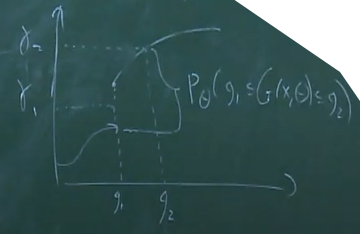
\includegraphics[height=6cm]{images/picture2.png}
\end{note}

\begin{note}
    Квантили $g_1$ и $g_2$ можно найти в статистических таблицах, либо с помощью функций из некоторых библиотек, их вычисляющих.
\end{note}

\begin{note}
    Не всегда центральную статистику можно найти методом пристального взгляда. Для таких случаев есть полезный результат.
\end{note}

\begin{lemma}
    Пусть $X_1, \dots, X_n$ -- независимые одинаково распределённые случайные величины с функцией распределения $F(x)$, $F(x)$ непрерывна. Тогда имеет место распределение:
    \[
        G(X_1, \dots, X_n) = -\sum_{i=1}^n \ln F(X_i) \sim \Gamma \ps{1, n}
    \]
\end{lemma}

\begin{proof}~
    \begin{itemize}
        \item $F(X_i) \sim U[0, 1]$

        Если функция распределения строго монотонна, в таком случае, с учётом непрерывности, она биективно отображает $\R$ на $(0, 1)$, то доказательство простое:
        \[
            \forall y \in (0, 1) \ \ P(F(X_i) \le y) = P(X_i \le F^{-1}(y)) = F(F^{-1}(y)) = y
        \]

        И получилось, что функция распределения $F(X_i)$ совпадает с функцией распределения $U[0,1]$. В общем случае это рассуждение нужно немного пофиксить:
        \[
            \forall y \in (0, 1) \ \ P(F(X_i) \le y) = P(X_i \le \max \{x : F(x) \le y\}) = F(\max \{x : F(x) \le y\}) = y
        \]

        Максимум достигается в силу того, что функция распределения непрерывна.

        \item $-\ln U[0, 1] \sim Exp(1)$

        Пусть $\xi \sim U[0, 1]$, тогда:
        \begin{align*}
            & \forall y > 0 \ \ P(-\ln \xi \le y) = P(\xi \ge e^{-y}) = 1 - P(\xi < e^{-y}) = [e^{-y} \in (0, 1)] = 1 - e^{-y}
            \\
            & P(-\ln \xi \le y) = (1 - e^{-y}) I\{y > 0\}
        \end{align*}

        Получили в точности функцию распределения $Exp(1)$.

        \item $G(X_1, \dots, X_n) \sim \Gamma \ps{1, n}$
        
        Применим накопленные знания, воспользовавшись также формулой для суммы независимых гамма-распределений:
        \[
            G(X_1, \dots, X_n) = -\sum_{i=1}^n \ln F(X_i) \sim -\sum_{i=1}^n \ln U[0, 1] \sim \sum_{i=1}^n Exp(1) \sim \sum_{i=1}^n \Gamma(1, 1) \sim \Gamma(1, n)
        \]
    \end{itemize}
\end{proof}

\begin{corollary}
    Если $X_1, \dots, X_n$ -- выборка из неизвестного распределения $P \in \{P_\theta,\ \theta \in \Theta\}$, причём для всех $\theta \in \Theta$ функция распределения $F_\theta(x)$ непрерывна по $x$, то $G(X_1, \dots, X_n, \theta) = -\sum_{i=1}^n \ln F_\theta(X_i)$ является центральной статистикой.
\end{corollary}

\subsection{Асимптотические доверительные интервалы}

\begin{definition}
    Пусть $(X_n,\ n \ge 1)$ --  выборка неограниченного размера из неизвестного распределения $P \in \{P_\theta,\ \theta \in \Theta\}$. Последовательность пар статистик
    \[
        (T_n^{(1)}(X_1, \dots, X_n), T_n^{(2)}(X_1, \dots, X_n))
    \]
    называется асимптотическим доверительным интервалом уровня доверия $\gamma$ для неизвестного параметра $\theta$, если
    \[
        \forall \theta \in \Theta \ \ \varliminf_{n \to \infty} P_\theta(T_n^{(1)}(\dots) < \theta < T_n^{(2)}(\dots)) \ge \gamma
    \]
    Если при этом
    \[
        \forall \theta \in \Theta \ \ \lim_{n \to \infty} P_\theta(T_n^{(1)}(\dots) < \theta < T_n^{(2)}(\dots)) = \gamma
    \]
    то асимптотический доверительный интервал называют точным.
\end{definition}

\begin{note}
    Нижний предел взяли из тех соображений, что обычный предел может не существовать, в том числе тогда, когда интервал с хорошей вероятностью оценивает параметр. В случае точного АДИ уже разумно брать обычный предел.
\end{note}

\begin{note}
    Асимптотический доверительный интервал можно построить с помощью асимптотически нормальной оценки. Пусть $\hat{\theta}_n(X_1, \dots, X_n)$ -- асимптотически нормальная оценка $\theta$ с асимптотической дисперсией $\sigma^2(\theta) > 0$, то есть:
    \begin{align*}
        & \forall \theta \ \ \sqrt{n}(\hat{\theta}_n - \theta) \xrightarrow{d_\theta} N(0, \sigma^2(\theta))
        \\
        & \forall \theta \ \ \sqrt{n} \frac{\hat{\theta}_n - \theta}{\sigma(\theta)} \xrightarrow{d_\theta} N(0, 1)
    \end{align*}

    Стандартно обозначим $u_\gamma$ -- $\gamma$-квантиль $N(0, 1)$, тогда в силу сходимости по распределению и того, что у $N(0, 1)$ функция распределения всюду непрерывна, получим:
    \[
        \lim_{n \to \infty} P_\theta \ps{-u_{\frac{1+\gamma}{2}} < \sqrt{n} \frac{\hat{\theta}_n - \theta}{\sigma(\theta)} < u_{\frac{1+\gamma}{2}}} = P_\theta \ps{-u_{\frac{1+\gamma}{2}} < N(0, 1) < u_{\frac{1+\gamma}{2}}} = \gamma
    \]

    Отсюда хочется выразить асимптотический доверительный интервал для $\theta$, но есть одна проблема: знаменатель $\sigma(\theta)$ зависит от $\theta$, поэтому просто выразить не получится. Исправим это, заменив $\sigma(\theta)$ на что-то, зависящее от выборки.

    Пусть $\sigma(\theta)$ непрерывна по $\theta$. Из асимптотической нормальности оценки следует её состоятельность, поэтому $\hat{\theta}_n \xrightarrow{P_\theta} \theta$ и в силу теоремы о наследовании сходимости $\sigma(\hat{\theta}_n) \xrightarrow{P_\theta} \sigma(\theta)$. Тогда по лемме Слуцкого:
    \[
        \forall \theta \ \ \sqrt{n} \frac{\hat{\theta}_n - \theta}{\sigma(\hat{\theta}_n)} = \sqrt{n} \frac{\hat{\theta}_n - \theta}{\sigma(\theta)} \cdot \frac{\sigma(\theta)}{\sigma(\hat{\theta}_n)} \xrightarrow{d_\theta} N(0, 1) \cdot 1 = N(0, 1)
    \]

    В таком случае, в соответствии с рассуждениями выше, можем получить асимптотический доверительный интервал для $\theta$ уровня доверия $\gamma$:
    \[
        \ps{\hat{\theta}_n - u_{\frac{1+\gamma}{2}} \frac{\sigma(\hat{\theta}_n)}{\sqrt{n}},\ \hat{\theta}_n + u_{\frac{1+\gamma}{2}} \frac{\sigma(\hat{\theta}_n)}{\sqrt{n}}}
    \]
\end{note}

\subsection{Метод максимального правдоподобия}

\begin{definition}
     Пусть $X$ -- выборка размера 1 из распределения $P \in \{P_\theta,\ \theta \in \Theta\}$, а семейство распределений $\{P_\theta,\ \theta \in \Theta\}$ доминируемо относительно меры $\mu$. Тогда функцией правдоподобия называется
     \[
        f_\theta(X) = p_\theta(X)
     \]
     Здесь $p_\theta(X)$ -- плотность $P_\theta$ по мере $\mu$. Важно, что функцию правдоподобия мы рассматриваем как функцию от $\theta$ при фиксированном $X$, а не наоборот. Функция правдоподобия, разумеется, не обязана быть вероятностной мерой на $\Theta$, это просто какая-то функция.
\end{definition}

\begin{example}
    Пусть $X = (X_1, \dots, X_n)$ -- выборка из распределения $P \in \{P_\theta,\ \theta \in \Theta\}$, семейство распределений $\{P_\theta,\ \theta \in \Theta\}$ доминируемо относительно меры $\mu$. Тогда функцией правдоподобия является
    \[
        f_\theta(X) = \prod_{i=1}^n p_\theta(X_i)
    \]

    Действительно, если рассматривать $X$ как случайный вектор из многомерного распределения, то именно функция $\prod_{i=1}^n p_\theta(x_i)$ будет плотностью этого распределения, что легко выводится из теоремы Фубини-Тонелли.
\end{example}

\begin{definition}
    Пусть $X$ -- выборка с функцией правдоподобия $f_\theta(X)$. Оценкой параметра $\theta$ по методу максимального правдоподобия (ОМП) называется такая статистика $\hat{\theta}(X)$, что
    \[
        \hat{\theta}(X) = \argmax_{\theta \in \Theta} f_\theta(X)
    \]
\end{definition}

\begin{note}
    Заметим, что в определение через термин статистика сразу закладываем измеримость. Соответственно, проблемы могут заключаться в том, что $\argmax$ может не существовать, быть не единственным, и не очевидна измеримость полученной функции.
\end{note}

\begin{example}
    Пусть есть монетка с распределением $Bern(p)$, причём известно что $p$ является одним из двух значений $p_1 = \frac{1}{9}$ или $p_2 = \frac{7}{8}$. Пусть есть выборка из трёх бросков монетки, запишем в виде $110$. Тогда посмотрим на вероятность такого события в случае разных $p$:
    \begin{align*}
        & p_1 \colon P_{p_1}(110) = \frac{1}{9} \cdot \frac{1}{9} \cdot \frac{8}{9}
        \\
        & p_2 \colon P_{p_2}(110) = \frac{7}{8} \cdot \frac{7}{8} \cdot \frac{1}{8}
    \end{align*}
    Во втором случае вероятность больше, то есть вторая модель более правдоподобна, гораздо лучше предсказывает то, что произошло в реальности. В этом и заключается идея оценки максимального правдоподобия.
\end{example}

\begin{example}
    Пусть есть выборка $X_1, \dots, X_n \sim U[0, \theta]$. Правдоподобие в таком случае имеет вид:
    \[
        f_\theta(X_1, \dots, X_n) = \frac{1}{\theta^n} \prod_{i=1}^n I\{0 \le X_i \le \theta\} = \frac{1}{\theta^n} \prod_{i=1}^n I\{0 \le X_{(1)} \le X_{(n)} \le \theta\}
    \]
    Тогда ОМП есть $\hat{\theta}(X) = X_{(n)}$.
\end{example}

\begin{note}
    Ту теорию, которую будем дальше развивать в этом разделе, можно также посмотреть в книге: Леман Теория точечного оценивания.
\end{note}

\begin{definition}
    Пусть $f_\theta(X)$ -- функция правдоподобия, тогда $L_\theta(X) = \ln f_\theta(X)$ называется логарифмической функцией правдоподобия. Так как плотность принимает значение ноль на элементах выборки с нулевой вероятностью, ибо интеграл от нуля равен нулю, то можем брать логарифм.
\end{definition}

\begin{definition}
    Нам вновь понадобятся условия регулярности. На этот раз их будет больше. Опять, сначала сформулируем, потом дадим пояснения.

    \begin{itemize}
        \item[(R0)] $\{P_\theta,\ \theta \in \Theta\}$ -- параметрическое семейство распределений, доминируемое относительно меры $\mu$, $P_{\theta_1} \neq P_{\theta_2}$ при $\theta_1 \neq \theta_2$. Для всех $\theta$ обозначим $p_\theta(x)$ -- плотность $P_\theta$ относительно меры $\mu$.

        \item[(R1)] Множество $A = \{x \in \cX \colon p_\theta(x) > 0\}$ не зависит от $\theta$, $A$ называется носителем.

        \item[(R2)] $X$ есть выборка из неизвестного распределения $P \in \{P_\theta,\ \theta \in \Theta\}$.

        \item[(R3)] $\Theta$ -- открытый интервал, возможно, бесконечный.

        \item[(R4)] Функция $p_\theta(x)$ непрерывно дифференцируема по $\theta$ при всех $x \in A$.

        \item[(R5)] Функция $p_\theta(x)$ трижды непрерывно дифференцируема по $\theta$ при всех $x \in A$.

        \item[(R6)] Интеграл $\int_A p_\theta(x) \mu(dx)$ трижды дифференцируем по $\theta$ под знаком интеграла.

        \item[(R7)] Информация Фишера $i(\theta) = \E_\theta \ps{\frac{\partial}{\partial \theta} \ln p_\theta(X_1)}^2 \in (0, +\infty)$

        \item[(R8)] $\forall \theta_0 \in \Theta \ \ \exists c > 0 \ \exists H(x) \ \ \forall \theta \in (\theta_0 - c, \theta_0 + c) \ \forall x \in A$ выполнено:
        \begin{align*}
            & \md{\frac{\partial^3}{\partial \theta^3} \ln p_\theta(x)} \le H(x)
            \\
            & \E_{\theta_0} H(X_1) < \infty
        \end{align*}        
    \end{itemize}
\end{definition}

\begin{note}
    Комментарии к некоторым условиям регулярности, те пояснения, которые были к условиям регулярности для эффективных оценок, дублировать не буду:
    \begin{itemize}
        \item[(R0)] Требование $P_{\theta_1} \neq P_{\theta_2}$ при $\theta_1 \neq \theta_2$ важно в следующем смысле, например, имеем семейство распределений $Bern(\theta^2)$ и поняли, что $\theta^2 = \frac{1}{4}$, отсюда никак не сможем сделать вывод о том, чему равно $\theta$, $\frac{1}{2}$ или $-\frac{1}{2}$.

        \item[(R2)] Просто зафиксировали выборку.

        \item[(R5)] Условие (R5), конечно, сильнее условия (R4), оба нужны, потому что в разных теоремах будут предполагаться разные условия регулярности. Сначала будут использоваться (R0)-(R2), как самые базовые, в которых осмыслено работать. Затем захотим дифференцировать по $\theta$, будем жить в условиях (R0)-(R4). Затем потребуется раскладывать функцию по формуле Тейлора до некоторого порядка, будут использоваться все условия (R0)-(R8).

        \item[(R6)] Полагаю, смысл следующий, дифференцируемость подинтегральных функций знаем из предыдущего пункта, здесь утверждение в том, что существуют конечные интегралы $\int_A p_\theta(x) \mu(dx)$, $\int_A \frac{\partial}{\partial \theta} p_\theta(x) \mu(dx)$, $\int_A \frac{\partial^2}{\partial \theta^2} p_\theta(x) \mu(dx)$, $\int_A \frac{\partial^3}{\partial \theta^3} p_\theta(x) \mu(dx)$.

        \item[(R8)] Здесь Савёлов сказал, что смысл станет понятен при доказательстве соответствующей теоремы, которую потом доказывать не стал. Тем не менее, сейчас некоторую интуицию для этого условия я приведу.
    \end{itemize}    
\end{note}

\begin{reminder} (Теорема о непрерывности собственного интеграла по параметру)
	Пусть $A \subseteq \R^n$, $E \subseteq \R^m$ --- измеримые множества и задана функция $f \colon E \times A \to \R$. Если наложены следующие условия:
	\begin{enumerate}
		\item Для любого $\alpha \in A$ функция $f(x, \alpha)$ измерима на $E$
		
		\item Почти всюду на $E$ выполнено $|f(x, \alpha)| \le \phi(x)$, где $\phi \in L_1(E)$
		
		\item Почти всюду на $E$ имеет место сходимость $f(x, \alpha) \to f(x, \alpha_0)$ при $\alpha \to \alpha_0$, $\alpha \in A$
	\end{enumerate}
	Тогда интеграл $\int_E f(x, \alpha)d\mu(x)$ непрерывен в точке $\alpha_0$, то есть имеется предел:
	\[
		\lim_{\alpha \to \alpha_0} \int_E f(x, \alpha)d\mu(x) = \int_E f(x, \alpha_0)d\mu(x)
	\]
\end{reminder}

\begin{note}
    Теперь поймём смысл (R8). Выведем из похожего условия (RR8), которое будет сформулировано ниже, в условиях регулярности (R0)-(R4) и (R7) непрерывность информации Фишера $i(\theta)$.
    
    Рассмотрим произвольную точку $\theta_0 \in \Theta$, хотим в ней доказать непрерывность функции:
    \[
        i(\theta) = \E_\theta \ps{\frac{\partial}{\partial \theta} \ln p_\theta(X_1)}^2 = \int_A \ps{\frac{\partial}{\partial \theta} \ln p_\theta(x)}^2 p_\theta(x) d\mu(x)
    \]

    Рассмотрим последний интеграл в некоторой окрестности $(\theta_0 - c, \theta_0 + c)$ точки $\theta_0$, чтобы доказать непрерывность в $\theta_0$, остальные $\theta$ нам не интересны. Хотим применить для множества $A \times (\theta_0 - c, \theta_0 + c)$, рассматривается $x \in A,\ \theta \in (\theta_0 - c, \theta_0 + c)$, и функции на нём $\ps{\frac{\partial}{\partial \theta} \ln p_\theta(x)}^2 p_\theta(x)$, теорему о непрерывности собственного интеграла по параметру, тогда получим в точности то, что хотим.

    Измеримость функции $\ps{\frac{\partial}{\partial \theta} \ln p_\theta(x)}^2 p_\theta(x)$ как функции от $x$ следует из того, что интеграл по ней, то есть информация Фишера, в силу (R7) существует и конечен. Непрерывность этой функции по $\theta$ следует из того, что в силу (R4) $p_\theta(x)$ непрерывно дифференцируема по $\theta$. Осталось мажорируемость интегрируемой функцией, для этого сформулируем условие (RR8):
    \begin{itemize}
        \item[(RR8)] $\forall \theta_0 \in \Theta \ \ \exists c > 0 \ \exists H(x) \ \ \forall \theta \in (\theta_0 - c, \theta_0 + c) \ \forall x \in A$ выполнено:
        \begin{align*}
            & \ps{\frac{\partial}{\partial \theta} \ln p_\theta(x)}^2 p_\theta(x) \le H(x)
            \\
            & \int_A H(x) \mu(dx) < \infty
        \end{align*}
    \end{itemize}

    Применяем теорему о непрерывности собственного интеграла по параметру, получаем, что информация Фишера $i(\theta)$ непрерывна в произвольной точке $\theta_0$, значит, непрерывна. Запомним этот факт, он нам ещё пригодится.

    Теперь сравним условия (R8) и (RR8):
    \begin{itemize}
        \item[(R8)] $\forall \theta_0 \in \Theta \ \ \exists c > 0 \ \exists H(x) \ \ \forall \theta \in (\theta_0 - c, \theta_0 + c) \ \forall x \in A$ выполнено:
        \begin{align*}
            & \md{\frac{\partial^3}{\partial \theta^3} \ln p_\theta(x)} \le H(x)
            \\
            & \E_{\theta_0} H(X_1) < \infty
        \end{align*}

        \item[(RR8)] $\forall \theta_0 \in \Theta \ \ \exists c > 0 \ \exists H(x) \ \ \forall \theta \in (\theta_0 - c, \theta_0 + c) \ \forall x \in A$ выполнено:
        \begin{align*}
            & \ps{\frac{\partial}{\partial \theta} \ln p_\theta(x)}^2 p_\theta(x) \le H(x)
            \\
            & \int_A H(x) \mu(dx) < \infty
        \end{align*}
    \end{itemize}

    В (R8) также мажорируется некоторая функция, конкретно, третья производная логарифмического правдоподобия, но рассматривается не интеграл от мажоранты, не зависящий от $\theta$, а интеграл от мажоранты по конкретной плотности, плотности меры $P_{\theta_0}$. Соответственно, беглый просмотр того доказательства, которое в этот раз не приводилось и в котором использовалось условие (R8) показал, что это условие там использовалось совершенно не так, как применялось здесь.    
\end{note}

\begin{theorem} (Экстремальное свойство правдоподобия)
    Пусть выполнены условия регулярности (R0)-(R2). Тогда
    \[
        \forall \theta_0, \theta \in \Theta,\ \theta_0 \neq \theta \ \ P_{\theta_0}(f_{\theta_0}(X_1, \dots, X_n) > f_\theta(X_1, \dots, X_n)) \xrightarrow[n \to \infty]{} 1 
    \]
\end{theorem}

\begin{note}
    В чём смысл теоремы: настоящий параметр $\theta_0$ становится правдоподобнее любого конкурента $\theta$, если увеличивать размер выборки.
\end{note}

\begin{lemma}
    Пусть $\{\xi_n\}_{n=1}^\infty$ -- независимые одинаково распределённые случайные величины. Пусть $\E\xi_1 \in \R \cup \{-\infty, +\infty\}$. Обозначим $S_n = \xi_1 + \dots + \xi_n$. Тогда
    \[
        \frac{S_n}{n} \xrightarrow{\text{п.н.}} \E\xi_1
.    \]
\end{lemma}

\begin{proof}
     Если $\E\xi_1$ конечно, то утверждение непосредственно следует из УЗБЧ. Рассмотрим случай $\E\xi_1 = +\infty$, случай $\E\xi_1 = -\infty$ рассматривается аналогично. Возьмём срезки от случайных величин $\xi_{n, [N]} = \min(\xi_n, N)$, тогда $\xi_{n, [N]}$ -- независимые одинаково распределённые случайные величины, $-\infty < \E\xi_{1, [N]} \le N < +\infty$. В силу УЗБЧ:
     \[
        \frac{S_{n, [N]}}{n} \xrightarrow{\text{п.н.}} \E\xi_{1, [N]}
     \]

     Теперь, применяя, что $\E\xi_{1, [N]} \xrightarrow[N \to \infty]{} +\infty$, так как $\E\xi_1 = +\infty$, получим:
     \[
        \frac{S_n}{n} \ge \frac{S_{n, [N]}}{n} \xrightarrow{\text{п.н.}} \E\xi_{1, [N]} \xrightarrow[N \to \infty]{} +\infty
     \]

     \color{gray}
     В целом, уже всё доказали, формально доводится следующим образом:
     \begin{align*}
         & \forall K \in \N \ \ P\ps{\varliminf_{n \to \infty} \frac{S_n}{n} \ge K} = 1
         \\
         & P\ps{\lim_{n \to \infty} \frac{S_n}{n} = +\infty} = P\ps{\bigcap_{K=1}^\infty \varliminf_{n \to \infty} \frac{S_n}{n} \ge K} = \lim_{K \to \infty} P\ps{\varliminf_{n \to \infty} \frac{S_n}{n} \ge K} = 1
     \end{align*}

     Совсем просто сделать нельзя, так как множества для сходимости почти наверное могут отличаться для разных $N$.
     \color{black}
\end{proof}

\begin{proof} (теоремы об экстремальном свойстве правдоподобия)
    Зафиксируем параметры $\theta_0 \neq \theta$. Можем считать, что все элементы выборки $X_1, \dots, X_n \in A$, т.е. имеют ненулевую плотность. Имеем на это право, ибо такое выполнено почти наверное для всех $P \in \{P_\theta,\ \theta \in \Theta\}$:
    \[
        P(\forall i \in \N \ X_i \in A) = P\ps{\bigcap_{i=1}^\infty \{X_i \in A\}} = \lim_{n \to \infty} P\ps{\bigcap_{i=1}^n \{X_i \in A\}} = \lim_{n \to \infty} 1 = 1
    \]
    
    Хотим доказать, что $P_{\theta_0}(f_{\theta_0}(X_1, \dots, X_n) > f_\theta(X_1, \dots, X_n)) \xrightarrow[n \to \infty]{} 1$. Можем переписать неравенство для функций правдоподобия в виде, к которому можно будет применить доказанную только что лемму об обобщённом УЗБЧ, здесь пользуемся тем, что плотность не равна нулю:
    \begin{align*}
        & f_{\theta_0}(X_1, \dots, X_n) > f_\theta(X_1, \dots, X_n)
        \\
        & \Updownarrow
        \\
        & \ln \frac{f_\theta(X_1, \dots, X_n)}{f_{\theta_0}(X_1, \dots, X_n)} < 0
        \\
        & \Updownarrow
        \\
        & \frac{1}{n} \sum_{i=1}^n \ln \frac{f_\theta(X_i)}{f_{\theta_0}(X_i)} < 0
    \end{align*}

    Далее хотим показать, что $-\infty \le \E_{\theta_0} \ln \frac{f_\theta(X_1)}{f_{\theta_0}(X_1)} < 0$. Если это так, то всё доказано, Савёлов это подробнее не обосновывал, мы распишем аккуратно, действительно, по лемме:
    \begin{align*}
        & P_{\theta_0}\ps{\lim_{n \to \infty} \frac{1}{n} \sum_{i=1}^n \ln \frac{f_\theta(X_i)}{f_{\theta_0}(X_i)} = \E_{\theta_0} \ln \frac{f_\theta(X_1)}{f_{\theta_0}(X_1)}} = 1
        \\
        & P_{\theta_0}\ps{\lim_{n \to \infty} \frac{1}{n} \sum_{i=1}^n \ln \frac{f_\theta(X_i)}{f_{\theta_0}(X_i)} < 0} = 1
        \\
        & P_{\theta_0}\ps{\exists N \ \forall n \ge N \ \ \frac{1}{n} \sum_{i=1}^n \ln \frac{f_\theta(X_i)}{f_{\theta_0}(X_i)} < 0} = 1
        \\
        & P_{\theta_0}\ps{\bigcup_{N=1}^\infty \bigcap_{n=N}^\infty \set{\frac{1}{n} \sum_{i=1}^n \ln \frac{f_\theta(X_i)}{f_{\theta_0}(X_i)} < 0}} = 1
    \end{align*}

    И отсюда получаем требуемую предельную вероятность: 
    \begin{multline*}
        \lim_{n \to \infty} P_{\theta_0}(f_{\theta_0}(X_1, \dots, X_n) > f_\theta(X_1, \dots, X_n)) = \lim_{n \to \infty} P_{\theta_0} \ps{\frac{1}{n} \sum_{i=1}^n \ln \frac{f_\theta(X_i)}{f_{\theta_0}(X_i)} < 0} \ge
        \\
        \ge \lim_{N \to \infty} P_{\theta_0} \ps{\bigcap_{n=N}^\infty \set{\frac{1}{n} \sum_{i=1}^n \ln \frac{f_\theta(X_i)}{f_{\theta_0}(X_i)} < 0}} = P_{\theta_0}\ps{\bigcup_{N=1}^\infty \bigcap_{n=N}^\infty \set{\frac{1}{n} \sum_{i=1}^n \ln \frac{f_\theta(X_i)}{f_{\theta_0}(X_i)} < 0}} = 1
    \end{multline*}

    Осталось доказать, что $\E_{\theta_0} \ln \frac{f_\theta(X_1)}{f_{\theta_0}(X_1)} < 0$. Для этого вспомним факт из математического анализа: $\ln(1+x) \le x$ при всех $x > -1$, равенство достигается только при $x = 0$. Дальнейшее доказательство будет состоять из серии хитрых и не очень преобразований:
    \begin{multline*}
        \E_{\theta_0} \ln \frac{f_\theta(X_1)}{f_{\theta_0}(X_1)} = \int_A \ln \frac{p_\theta(x)}{p_{\theta_0}(x)} p_{\theta_0}(x) \mu(dx) = \int_A \ln \ps{1 + \frac{p_\theta(x)}{p_{\theta_0}(x)} - 1} p_{\theta_0}(x) \mu(dx) \le
        \\
        \le \int_A \ps{\frac{p_\theta(x)}{p_{\theta_0}(x)} - 1} p_{\theta_0}(x) \mu(dx) = \int_A \ps{p_\theta(x) - p_{\theta_0}(x)} \mu(dx) = 1 - 1 = 0
    \end{multline*}

    Пока доказали нестрогую версию неравенства, $\E_{\theta_0} \ln \frac{f_\theta(X_1)}{f_{\theta_0}(X_1)} \le 0$, но равенство может быть лишь в случае $\frac{p_\theta(x)}{p_{\theta_0}(x)} - 1 = 0 \ \mu\text{-п.н.} \Lra p_\theta(x) = p_{\theta_0}(x) \ \mu\text{-п.н.}$, то есть $P_{\theta_0} = P_\theta$, тогда $\theta = \theta_0$ в силу одного из условий регулярности, что невозможно в силу выбора $\theta \neq \theta_0$.
\end{proof}